% !TeX spellcheck = en_US
\section{Atlassian Jira Agile}
\subsection{What does Jira Agile provide?}

Jira Agile provides task management support for the two main agile methodologies
SCRUM and Kanban. It focuses on creating and managing tasks, issues, stories,
epics and bug reports. Developers can estimate and prioritize these planning
cards. Administrators define task flow processes according to certain filters
and constraints. All developers must follow these rules afterward. The whole
Jira framework is highly adaptable and configurable to future needs, i.e. new
Kanban board columns and statuses can be defined and multiple projects can be
visualized all at once on a configurable dashboard. It also integrates with
Jira, Confluence and other development tools. 

Another feature is the integration with source code revision tools, like Git,
SVN and Bitbucket. It bridges the gap between user stories and source code
commits.

On the side of analysis, Jira Agile does not offer a lot. At least build-in
features are scarce. If developers use Kanban, they can monitor current trends
and analyze past progresses. The tool that visualizes this metrics is called
cumulative flow diagram, please refer to figure~\ref{fig:cumulative_flow_diagram}. 
I think, this could be a good
point where PROM comes in with analysis tools. Maybe we could add effort metrics
and product metrics here. For instance, CC, LLOC, and LCOM4. It could be even
feasible to integrate SonarQube features here, maybe we could add them first to
PROM services, or provide an unified interface to PROM and SonarQube metrics and
statistics through a REST service or something similar.

\begin{figure}[h]
	\centering
	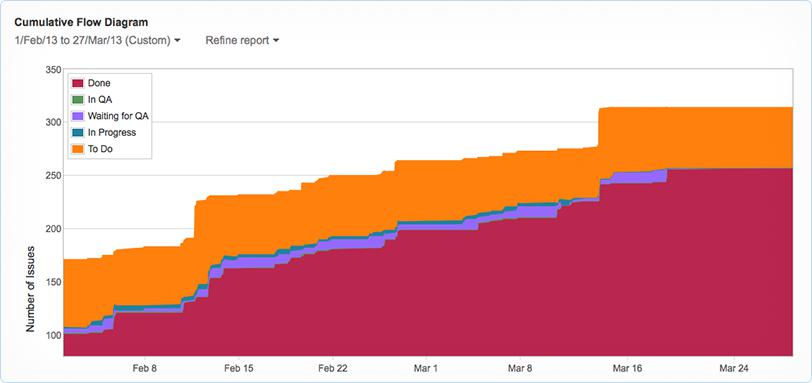
\includegraphics[scale=0.5]{img/cumulative_flow_diagram.jpg}
	\caption{Cumulative flow diagram with number of issues over time.} 
	\label{fig:cumulative_flow_diagram}
\end{figure}